\documentclass[aspectratio=149, xcolor=table]{beamer}
\usetheme{Montpellier}
\usefonttheme{serif}
\usecolortheme{dove}
\useinnertheme{rounded}
\setbeamersize{text margin left=5mm,text margin right=10mm}
\usefonttheme{serif}
\usepackage{graphicx}
\usepackage[italian]{babel}
\usepackage[utf8]{inputenc}
\usepackage{tabularx}
\usepackage{tikz}
\usepackage[absolute,overlay]{textpos} 
\usepackage{xcolor}
\usepackage{multicol}
\definecolor{myGreen}{RGB}{54, 114, 89}
\definecolor{unipd}{RGB}{155, 0, 20}
\definecolor{sbj1}{HTML}{77AC30}
\definecolor{sbj2}{HTML}{EDB120}
\definecolor{sbj3}{HTML}{0072BD}
\definecolor{sbj4}{HTML}{1F78B4}
\definecolor{sbj5}{HTML}{33A02C}
\definecolor{sbj6}{HTML}{E31A1C}
% Per il tema Montpellier
%\setbeamercolor{separation line}{bg=myGreen!20}
\setbeamercolor{separation line}{bg=black!20}
%\setbeamercolor{title in head/foot}{bg=white, fg=myGreen}
\setbeamercolor{title in head/foot}{bg=white, fg=black}
%\setbeamercolor{section in head/foot}{bg=white, fg=myGreen}
%\setbeamercolor{subsection in head/foot}{bg=white, fg=myGreen}
%\setbeamercolor{background canvas}{bg=white}
%\setbeamercolor{title}{fg=myGreen}
%\setbeamercolor{item}{fg =myGreen}
%\setbeamercolor{frametitle}{fg = myGreen}
%\setbeamercolor{section in toc}{fg=myGreen!80}
%\setbeamercolor{subsection in toc}{fg=black}
\setbeamerfont{section in toc}{series=\bfseries,size=\normalsize}
\setbeamerfont{frametitle}{series=\bfseries}
%\setbeamerfont{title}{family=\scshape}
%\setbeamercolor{frametitle}{fg=unipd}
%\setbeamercolor{section in head/foot}{bg=unipd, fg=white}
%\setbeamercolor{subsection in head/foot}{fg=unipd}
%\setbeamercolor{author in head/foot}{bg=unipd, fg=white}
%\setbeamercolor{title in head/foot}{fg=unipd}
%\setbeamercolor{date in head/foot}{fg=unipd}

% definisce gli elementi da mettere sopra la figura 
% rectangles on figures 
\newcommand{\imagenode}[2][1]% [scale], filename
{   \node[above right,inner sep=0] (myimage) {\includegraphics[scale=#1]{#2}};
	\path (myimage.north east);
	\pgfgetlastxy{\myimagex}{\myimagey}
	\pgfmathsetmacro{\myimagewidth}{\myimagex/28.453}
	\pgfmathsetmacro{\myimageheight}{\myimagey/28.453}
}
\newcommand{\imagegrid}[4][help lines]% [options], steps, font, precision
{   \pgfkeys{/pgf/number format/.cd,fixed,precision=#4}
	\foreach \x in {0,...,#2}
	{   \draw[#1] (\x/#2*\myimagewidth,\myimageheight) -- (\x/#2*\myimagewidth,0) node[below] {#3\pgfmathparse{\x/#2}\pgfmathprintnumber{\pgfmathresult}};
		\draw[#1] (\myimagewidth,\x/#2*\myimageheight) -- (0,\x/#2*\myimageheight) node[left] {#3\pgfmathparse{\x/#2}\pgfmathprintnumber{\pgfmathresult}};
	}
}

\newcommand{\highlightbox}[8][densely dashed,thick]% [options], left, low, right, up, node options, node text, overlay spec
{   \only<#8>{\draw[#1] (#2*\myimagewidth, #3*\myimageheight) rectangle node[#6] {#7} (#4*\myimagewidth, #5*\myimageheight);}
}

\newcommand{\highlighttext}[8][densely dashed,thick]% [options], left, low, right, up, node options, node text, overlay spec
{   \only<#8>{\path[#1] (#2*\myimagewidth, #3*\myimageheight) rectangle node[#6] {#7} (#4*\myimagewidth, #5*\myimageheight);}
}

% tikz per la cfa 

\usetikzlibrary{shapes.geometric, arrows}
\tikzstyle{latent} = [ellipse, minimum width=2.5cm, minimum height=2cm,text centered, draw=black]
\tikzstyle{item} = [rectangle, rounded corners, minimum width=0.5cm, minimum height=1cm, text width =1.5cm, text centered, draw=black]
\tikzstyle{arrow} = [thick,->,>=stealth]

% allegedly, il codice che viene dopo permette di cambiare colore alle celle 

\makeatletter
\def\rowcolor{\noalign{\ifnum0=`}\fi\bmr@rowcolor}
\newcommand<>{\bmr@rowcolor}{%
	\alt#1%
	{\global\let\CT@do@color\CT@@do@color\@ifnextchar[\CT@rowa\CT@rowb}% 
	{\ifnum0=`{\fi}\@gooble@rowcolor}% 
}

\newcommand{\@gooble@rowcolor}[2][]{\@gooble@rowcolor@}
\newcommand{\@gooble@rowcolor@}[1][]{\@gooble@rowcolor@@}
\newcommand{\@gooble@rowcolor@@}[1][]{\ignorespaces}
\makeatother



\makeatletter
\def\cellcolor{{\ifnum0=`}\fi\bmr@cellcolor}
\newcommand<>{\bmr@cellcolor}{%
	\alt#1%
	{\global\let\CT@do@color\CT@@do@color\@ifnextchar[\CT@rowa\CT@rowb}% 
	{\ifnum0=`{\fi}\@gooble@cellcolor}% 
}

\newcommand{\@gooble@cellcolor}[2][]{\@gooble@cellcolor@}
\newcommand{\@gooble@cellcolor@}[1][]{\@gooble@cellcolor@@}
\newcommand{\@gooble@cellcolor@@}[1][]{\ignorespaces}
\makeatother

\AtBeginSection[]
{
	\begin{frame}
		\tableofcontents[currentsection, currentsubsection]
	\end{frame}
}

\AtBeginSubsection[]
{
	\begin{frame}
		\tableofcontents[currentsection, currentsubsection]
	\end{frame}
}


\title[Meaningfulness]{Le misure in psicologia sono significanti?\\ Il caso del test della Torre di Londra}
\author[Epifania et al.]{\textbf{Ottavia M. Epifania}, Luca Stefanutti, Pasquale Anselmi,  Andrea Brancaccio, Debora de Chiusole}
\institute [UniPd] {
	
\includegraphics[width=10mm]{unipd.png}\\ 
Dipartimento di Filosofia, Sociologia, Pedagogia e Psicologia Applicata,\\	Università di Padova}
	
	\date [AIP2023] {%\vspace{0.6cm}\\
		Convegno AIP-Sezione Sperimentale 2023\\ Simposio: Crisi di replicabilità o crisi di validità? L’importanza delle misure \\ \vspace{3mm}
		19 Settembre 2023}
\begin{document}
	
	\begin{frame}[plain]
		\maketitle
	\end{frame}

\section{Meaningfulness}


\begin{frame}
	
	The ratio between the measures of $a$ and $b$ is constant and independent of the measurement unit:
	\[
	\frac{\varphi(a)}{\varphi(b)} = \frac{\varphi'(a)}{\varphi'(b)},
	\]
	
	where $\varphi$ and $\varphi'$ are two different scales of measurement of the same variable.
	
	\pause
	\begin{block}{Meaningful comparisons}
		
		The comparison between \emph{a} and \emph{b} is meaningful if it is invariant under all the unit transformations. 
			
	\end{block}
\end{frame}

\begin{frame}
	
	\begin{tikzpicture}
		% load the first image nature1.png as a node called img1
		\node (img1) {
\includegraphics[width=\linewidth]{img/time.png}};
		\pause
		\node[opacity=0.8]  (img2) at (img1.center)
		{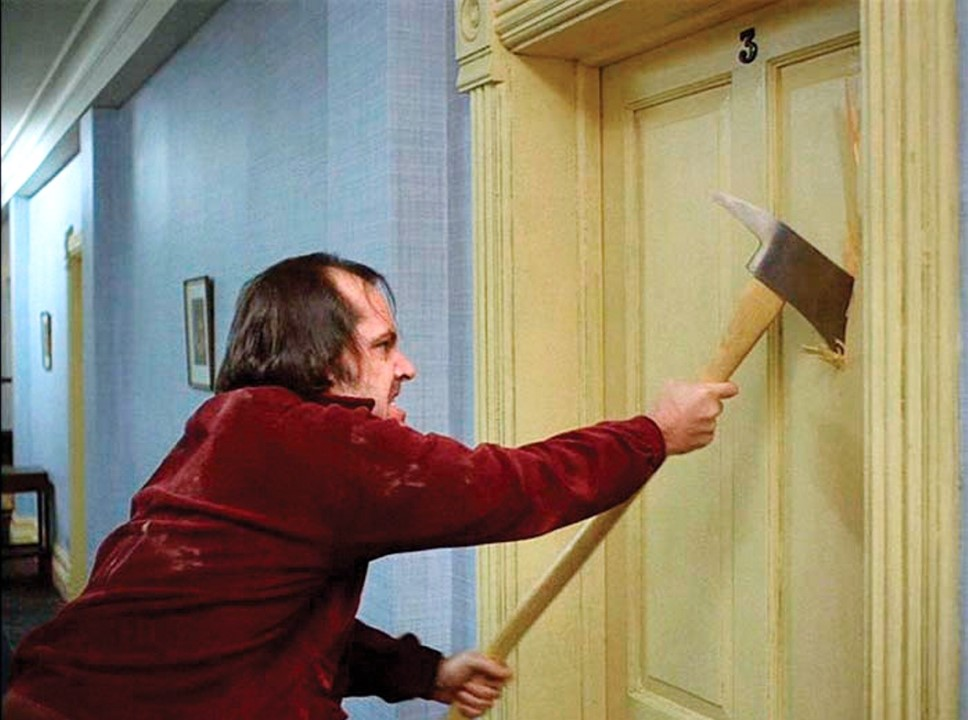
\includegraphics[width=.70\linewidth]{img/jt_axe.jpg}};
	\end{tikzpicture}
	
	
\end{frame}

\section{The case in point}
\subsection{Tower of London}
\begin{frame}
	
	\begin{columns}
		\column{0.45\textwidth}
		\begin{center}
			\begin{tikzpicture}[scale=1.2]
				\node (start) [mark=diamond,inner sep = 0pt, minimum size = 4pt] (23) at (  -1.5,  3.5*1.73) {
					\begin{tikzpicture}[scale=.6]
						\draw[draw=black!20,fill=black!20] (0,5) rectangle (6,5.3);
						\draw[draw=black!20,fill=black!20] (0.85,5) rectangle (1.15,8.5);
						\draw[draw=black!20,fill=black!20] (2.85,5) rectangle (3.15,7.5);
						\draw[draw=black!20,fill=black!20] (4.85,5) rectangle (5.15,6.5);
						\draw[fill=red] (1,5.8) circle (15pt);
						\draw[fill=yellow] (5,5.8) circle (15pt);
						\draw[fill= blue] (3,5.8) circle (15pt);
					\end{tikzpicture}
				};
			\end{tikzpicture}\\
			Starting configuration
		\end{center}
		\column{0.45\textwidth}
		\begin{center}
			\begin{tikzpicture}[scale=1.2]
				\node (goal) [mark=diamond,inner sep = 0pt, minimum size = 4pt] (23) at (  -1.5,  3.5*1.73) {
					\begin{tikzpicture}[scale=.6]
						\draw[draw=black!20,fill=black!20] (0,5) rectangle (6,5.3);
						\draw[draw=black!20,fill=black!20] (0.85,5) rectangle (1.15,8.5);
						\draw[draw=black!20,fill=black!20] (2.85,5) rectangle (3.15,7.5);
						\draw[draw=black!20,fill=black!20] (4.85,5) rectangle (5.15,6.5);
						\draw[fill=yellow] (1,5.8) circle (15pt);
						\draw[fill=red] (1,6.85) circle (15pt);
						\draw[fill=blue] (3,5.8) circle (15pt);
					\end{tikzpicture}
				};
				
			\end{tikzpicture}\\
			Goal configuration 
		\end{center}
	\end{columns}
	\pause
	\vspace{3mm}
	
	Item difficulty influenced by: 
	
	\begin{itemize}
		\item Number of moves
		\item Number of alternative paths
		\item Hierarchy of the starting/goal configuration
	\end{itemize}
	
	

	

\end{frame}




\begin{frame}{The Tower of London Test (ToL Test) }{Shallice (1982)}
	\begin{columns}[T]
		\column{0.45\textwidth}
		
		\begin{center}
			\small
			\begin{itemize}
				\item 12 problems    
				\vspace{.2cm}
				\item Same starting configuration
				\vspace{.2cm}
				\item More than one attempt per item 
			\end{itemize}
			
			\vspace{.3cm}
			\begin{tikzpicture}[scale=1.2]
				\node[mark=diamond,inner sep = 0pt, minimum size = 4pt] (23) at (  -1.5,  3.5*1.73) {
					\begin{tikzpicture}[scale=.4]
						\draw[draw=black!20,fill=black!20] (0,5) rectangle (6,5.3);
						\draw[draw=black!20,fill=black!20] (0.85,5) rectangle (1.15,8.5);
						\draw[draw=black!20,fill=black!20] (2.85,5) rectangle (3.15,7.5);
						\draw[draw=black!20,fill=black!20] (4.85,5) rectangle (5.15,6.5);
						\draw[fill=yellow] (1,5.8) circle (15pt);
						\draw[fill=red] (1,6.85) circle (15pt);
						\draw[fill=blue] (3,5.8) circle (15pt);
					\end{tikzpicture}
				};
			\end{tikzpicture}
		\end{center}
		
		\column{0.45\textwidth}
		\vspace{- .5cm}
		\begin{center}    
			\scriptsize
			
			\scalebox{.80}{
				\begin{tabular}{ccc}
				\hline
				Problem	&	Minimum moves	&	Alternative paths	\\
				\hline
				Example	&	2	&	1	\\
				1	&	2	&	1	\\
				2	&	2	&	1	\\
				3	&	3	&	2	\\
				4	&	3	&	1	\\
				5	&	4	&	2	\\
				6	&	4	&	1	\\
				7	&	4	&	1	\\
				8	&	4	&	1	\\
				9	&	5	&	2	\\
				10	&	5	&	1	\\
				11	&	5	&	1	\\
				12	&	5	&	2	\\
				\hline
			\end{tabular}
			}

		
		\end{center}
	\end{columns}
\end{frame}

\subsection{Scoring systems}

\begin{frame}


\centering
\scalebox{.80}{

\begin{tabular}{l c c c c}
\hline
Scoring & Attempts & Response times & Item score & Total score \\\hline
\textcolor<2->{black!15}{Shallice 1} & \textcolor<2->{black!15}{$\checkmark$} & \textcolor<2->{black!15}{$\checkmark$} & \textcolor<2->{black!15}{0-1} & \textcolor<2->{black!15}{0-12} \\
 \cellcolor<2>{black!20}Shallice 2 & $\times$ & $\checkmark$ &0-3 & 0-36\\
 \cellcolor<2>{black!20}Anderson et al. & $\checkmark$ & $\checkmark$ & 0-9& 0-108 \\
\textcolor<2->{black!15}{Kirkorian et al.} & \textcolor<2->{black!15}{$\checkmark$} & \textcolor<2->{black!15}{$\times$} & \textcolor<2->{black!15}{0-3}& \textcolor<2->{black!15}{0-36} \\\hline


\end{tabular}
}


\vspace{-1.5mm}
\onslide<2->
\begin{columns}[T]
	\begin{column}{.50\linewidth}
		\begin{center}
			Shallice 2 -- SH2
		\end{center}
		\small
			 For each of the 12 items:
			\bigskip
			
			\centering
			\begin{tabular}{cc}
				\hline
				Assign & if time is\\
				\hline
				3 & $\leq 15$ s \\
				2 & $15 \dashv 30$ s \\
				1 & $30 \dashv 60$ s \\
				0 & $>60$ s \\
				\hline
			\end{tabular}
			\bigskip
			
	\end{column}
	
		\begin{column}{.50\linewidth}
			\begin{center}
			Anderson et al. -- AN
		\end{center}
		\small
		\centering
			 For each of the 12 items:
				\bigskip			
				
			\begin{tabular}{cl}
				\hline
				Assign & if time is\\
				\hline
				9 & $\leq6$ s \\
				8 & $6\dashv10$ s \\
				7 & $11\dashv20$ s \\
				6 & $21\dashv40$ s \\
				5 & $41\dashv60$ s \\
				0 & $>60$ s \\
				\hline
			\end{tabular}
			\footnotesize \normalfont 
			\flushleft
			
			Subtract the number of unsuccessful attempts
	\end{column}
\end{columns}
\end{frame}

\begin{frame}
	Both scorings are based on the discretization of the response times  $\rightarrow$ There should not be differences in the \textbf{order} of the total score of the respondents according to the scoring method 
	
	%\begin{center}
	%
\includegraphics[width=.03\linewidth]{img/arrowDown.png}
	%\end{center}
	
	
	
	\pause
	
	\begin{figure}
	\centering
	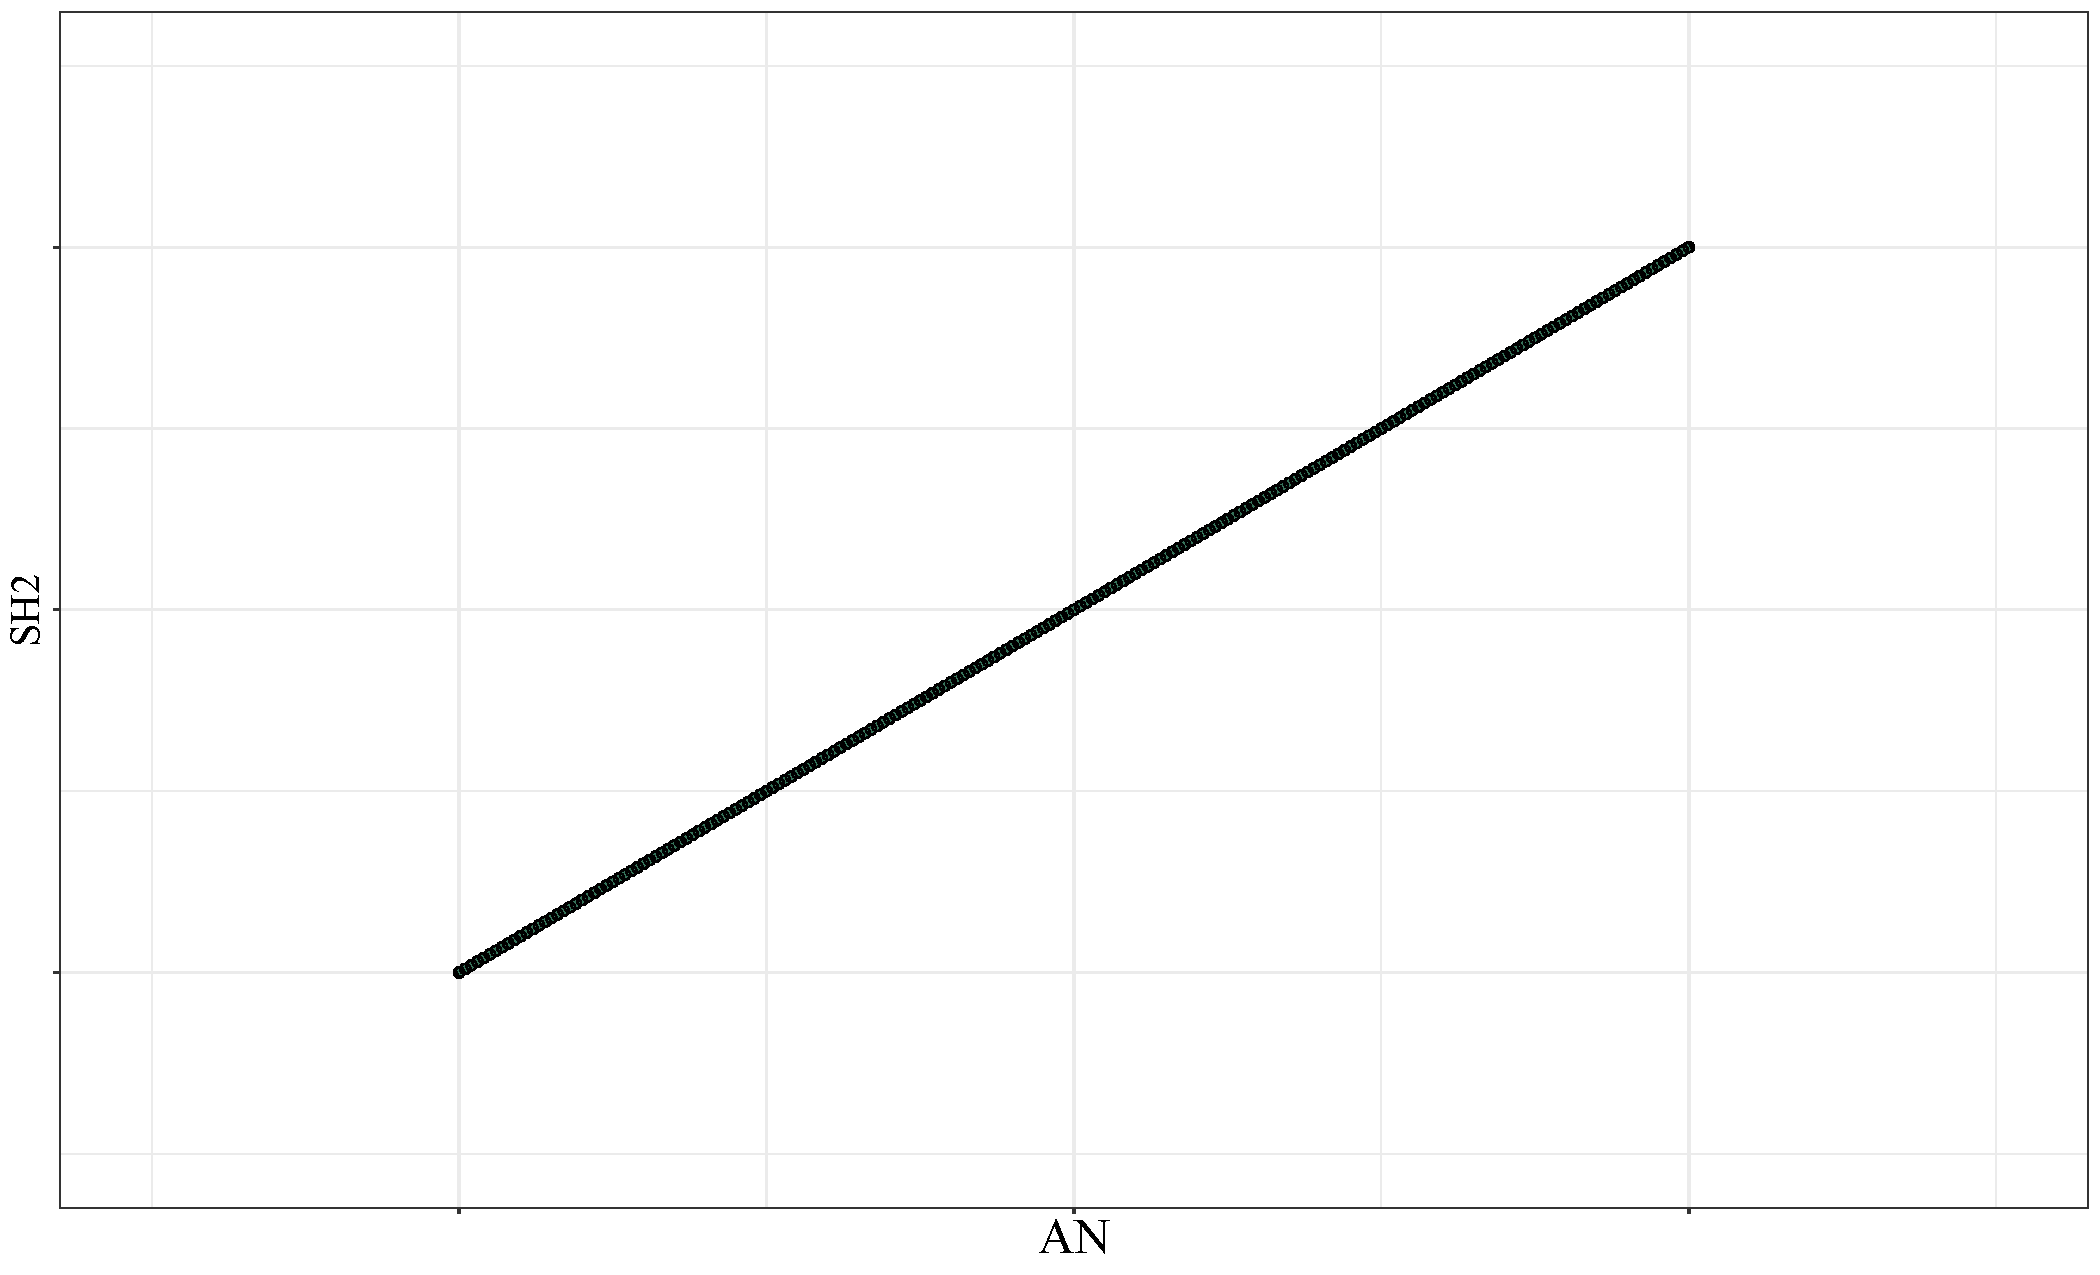
\includegraphics[width=.70\linewidth]{img/exp.pdf}
	\end{figure}
	
	\end{frame}



\section{Real data application}
	

	
%	\begin{frame}
%	
%		$n = 343$
%	\begin{figure}
%	\centering
%	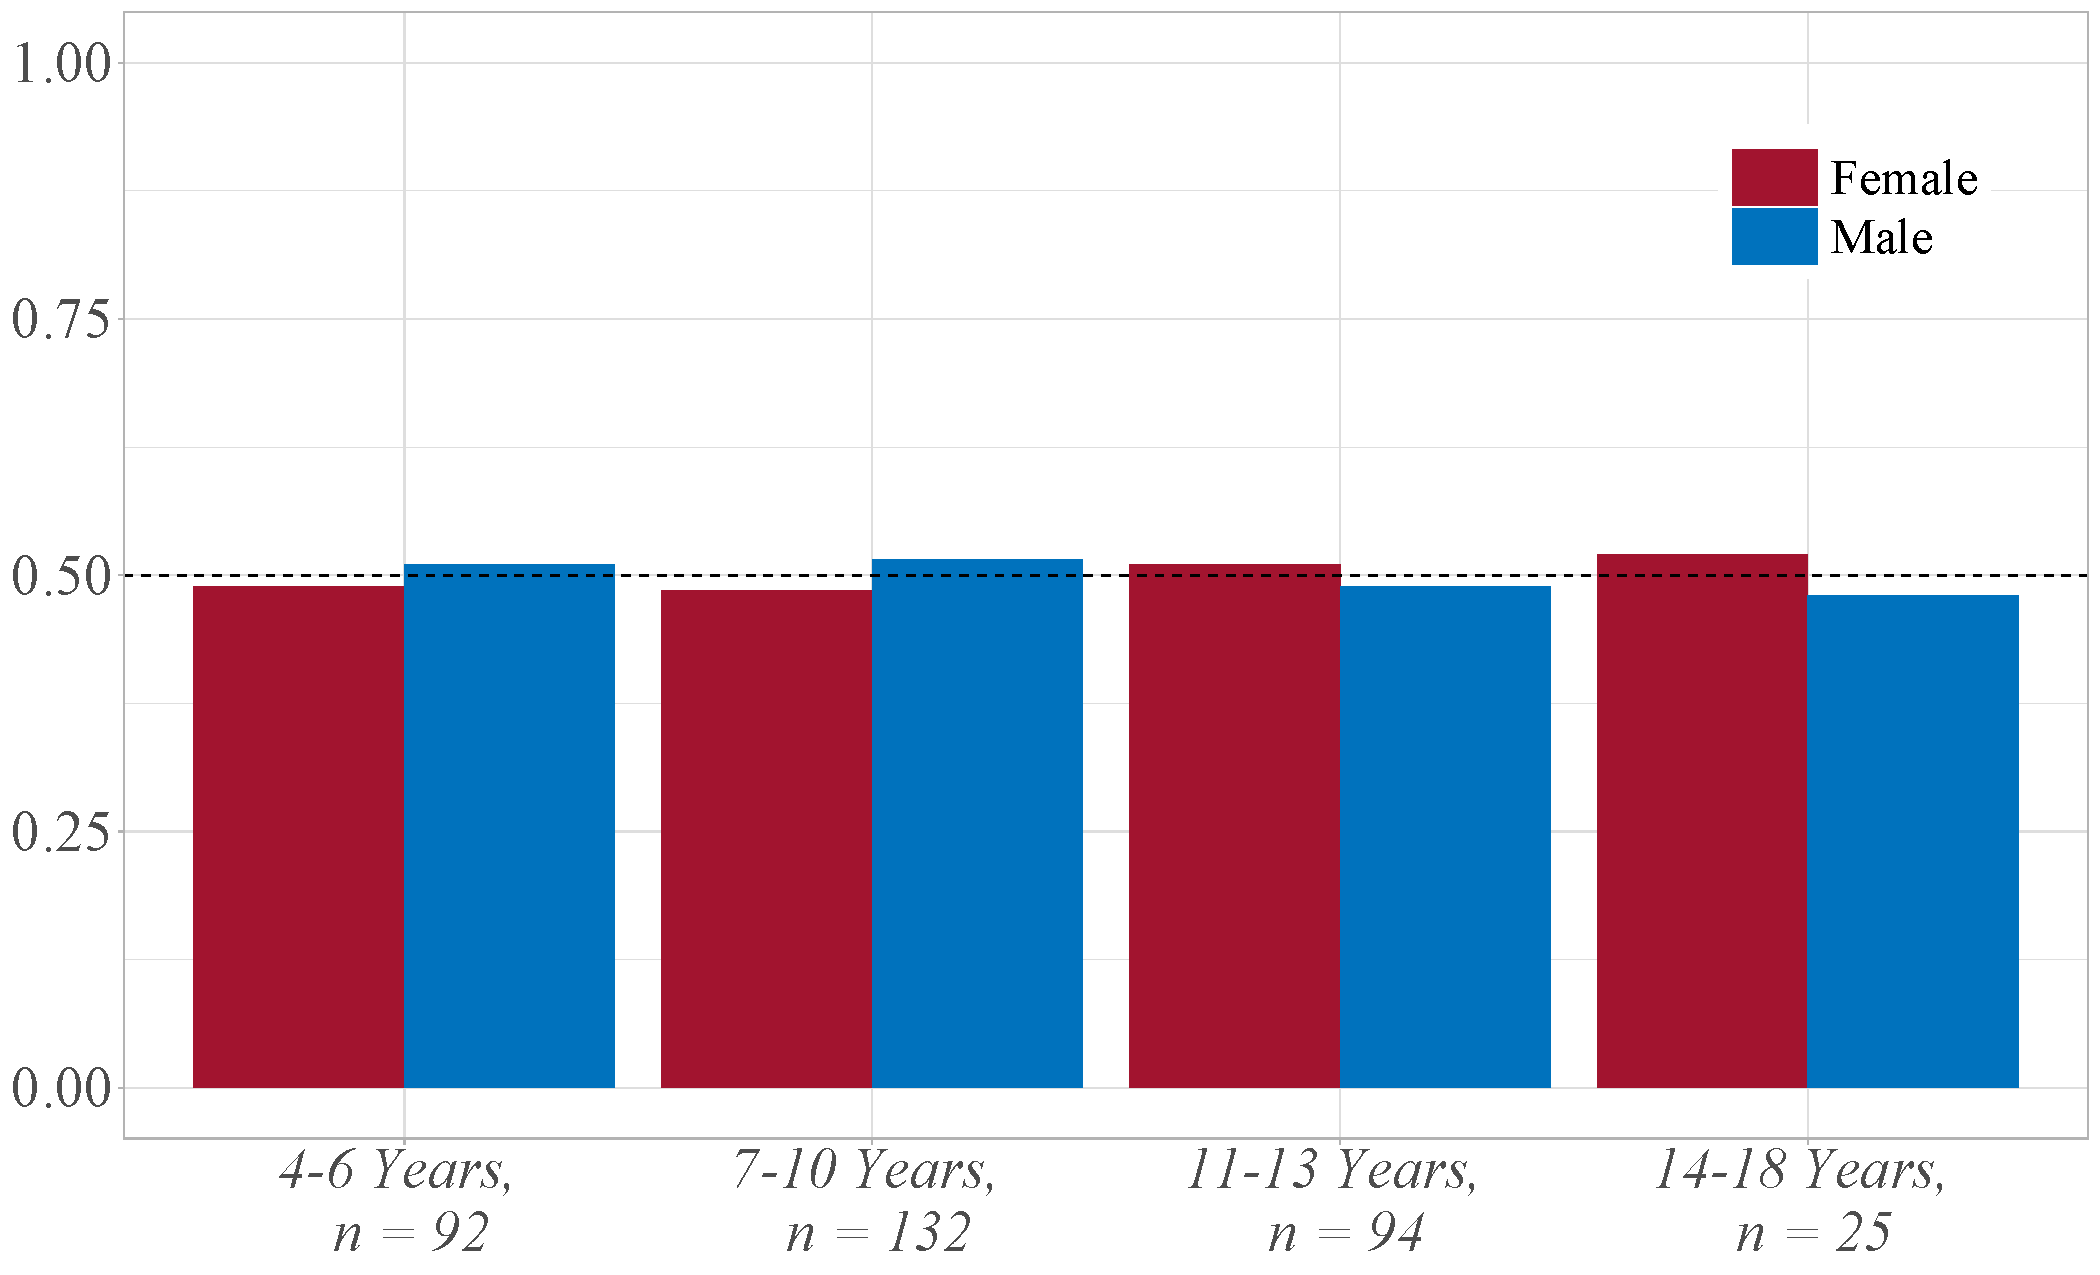
\includegraphics[width=.85\linewidth]{img/descrittive_gender.pdf}
%	\end{figure}
%	\end{frame}
	
	
%	\begin{frame}
%		
%		$n = 343$, F $= 49$\%
%		
%		 
%	
%	\begin{columns}
%	
%	\begin{column}{.50\linewidth}
%	
%	\begin{center}
%	Accuracy score
%	\end{center}
%		\centering
%	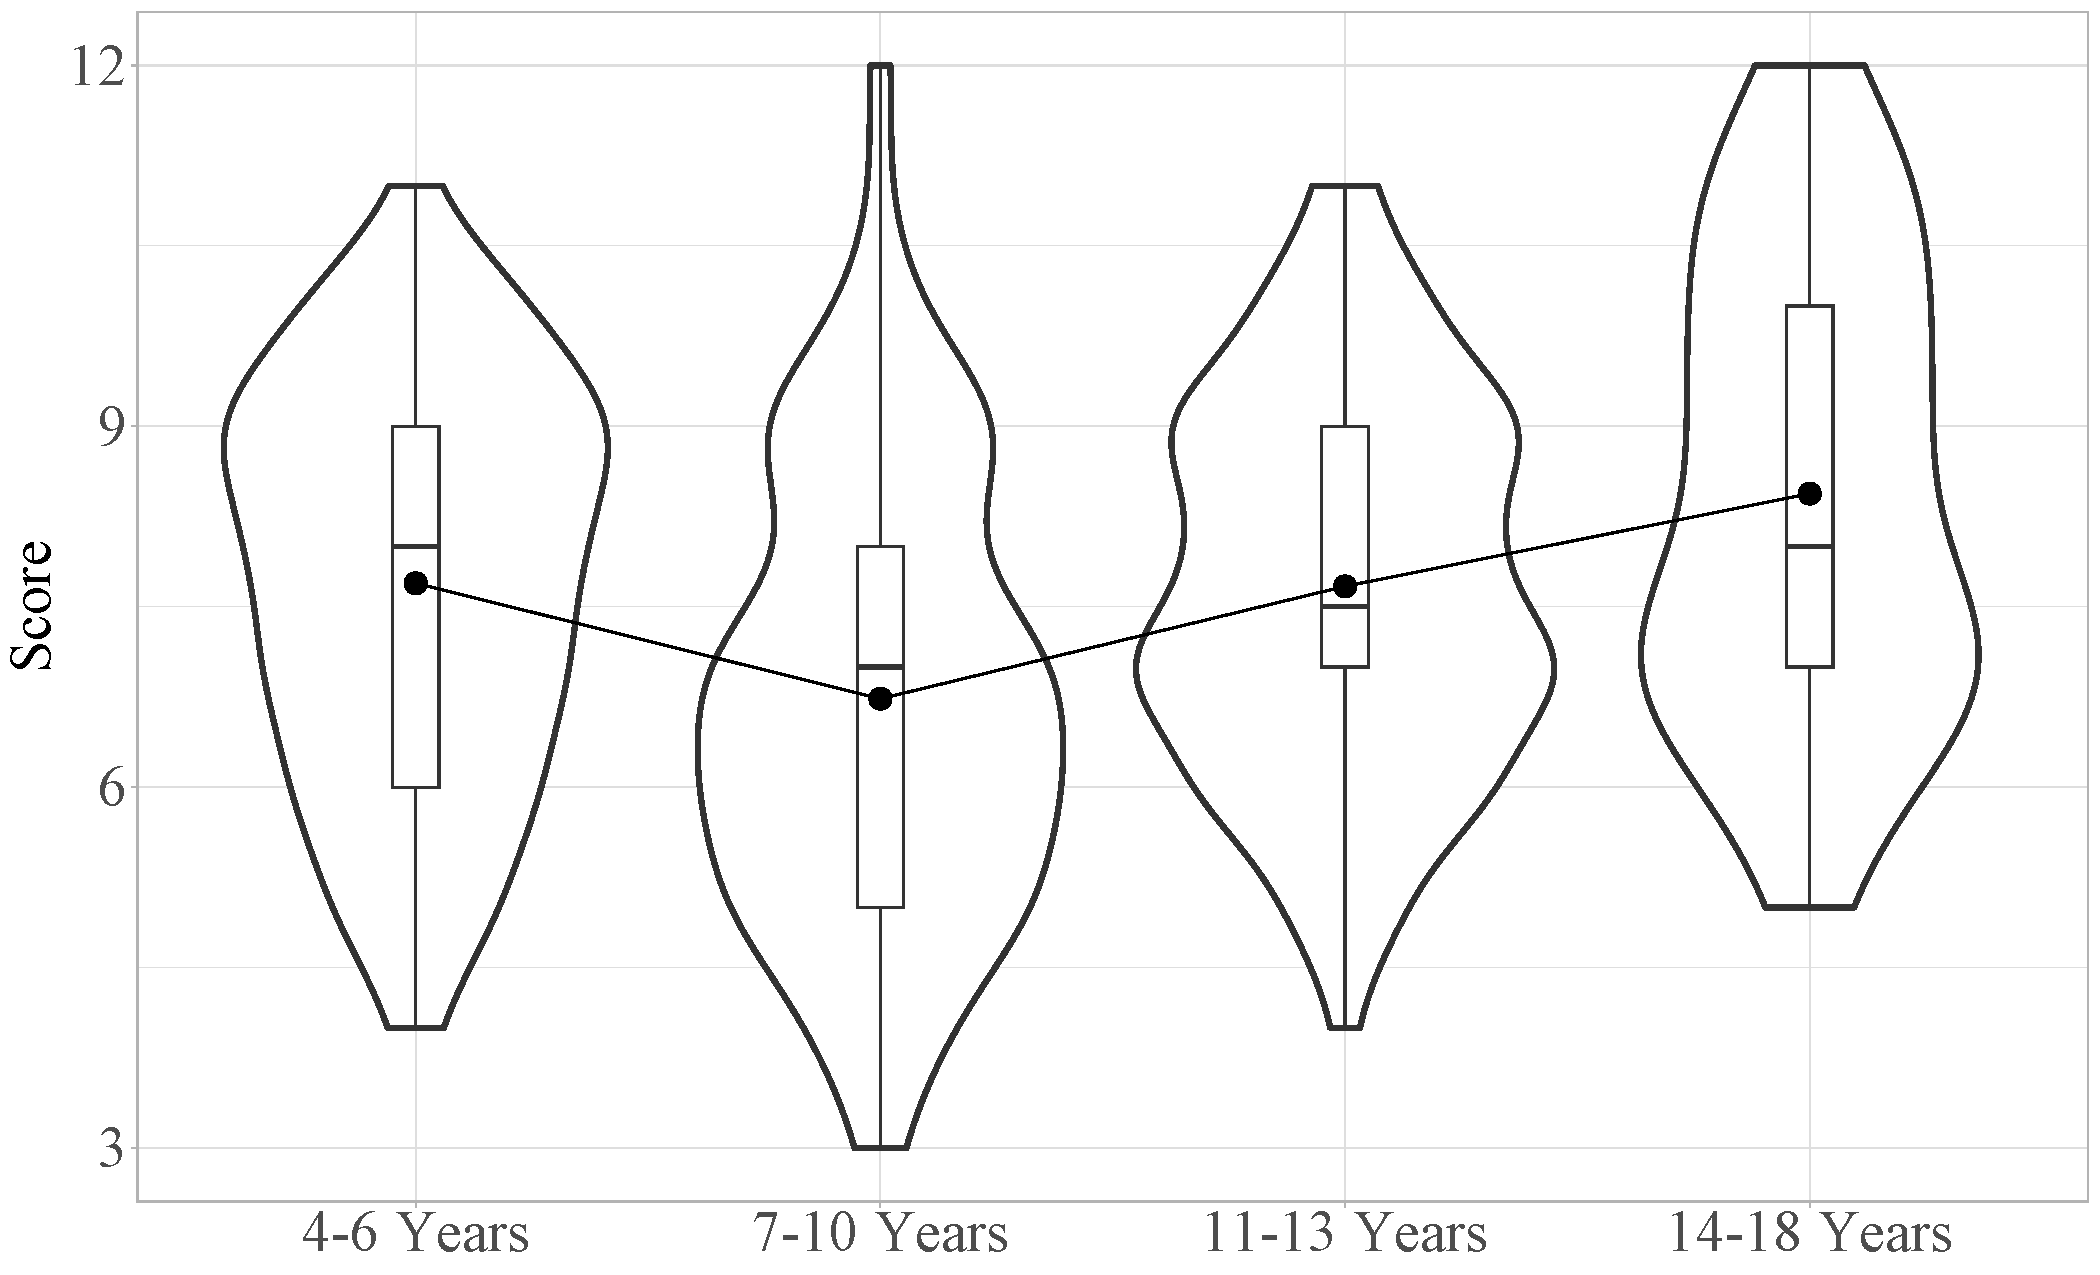
\includegraphics[width=\linewidth]{img/descrittive_accuratezze.pdf}
%		
%	\end{column}
%	
%		\begin{column}{.50\linewidth}
%		
%			\begin{center}
%	Response times
%	\end{center}
%		\centering
%		
%			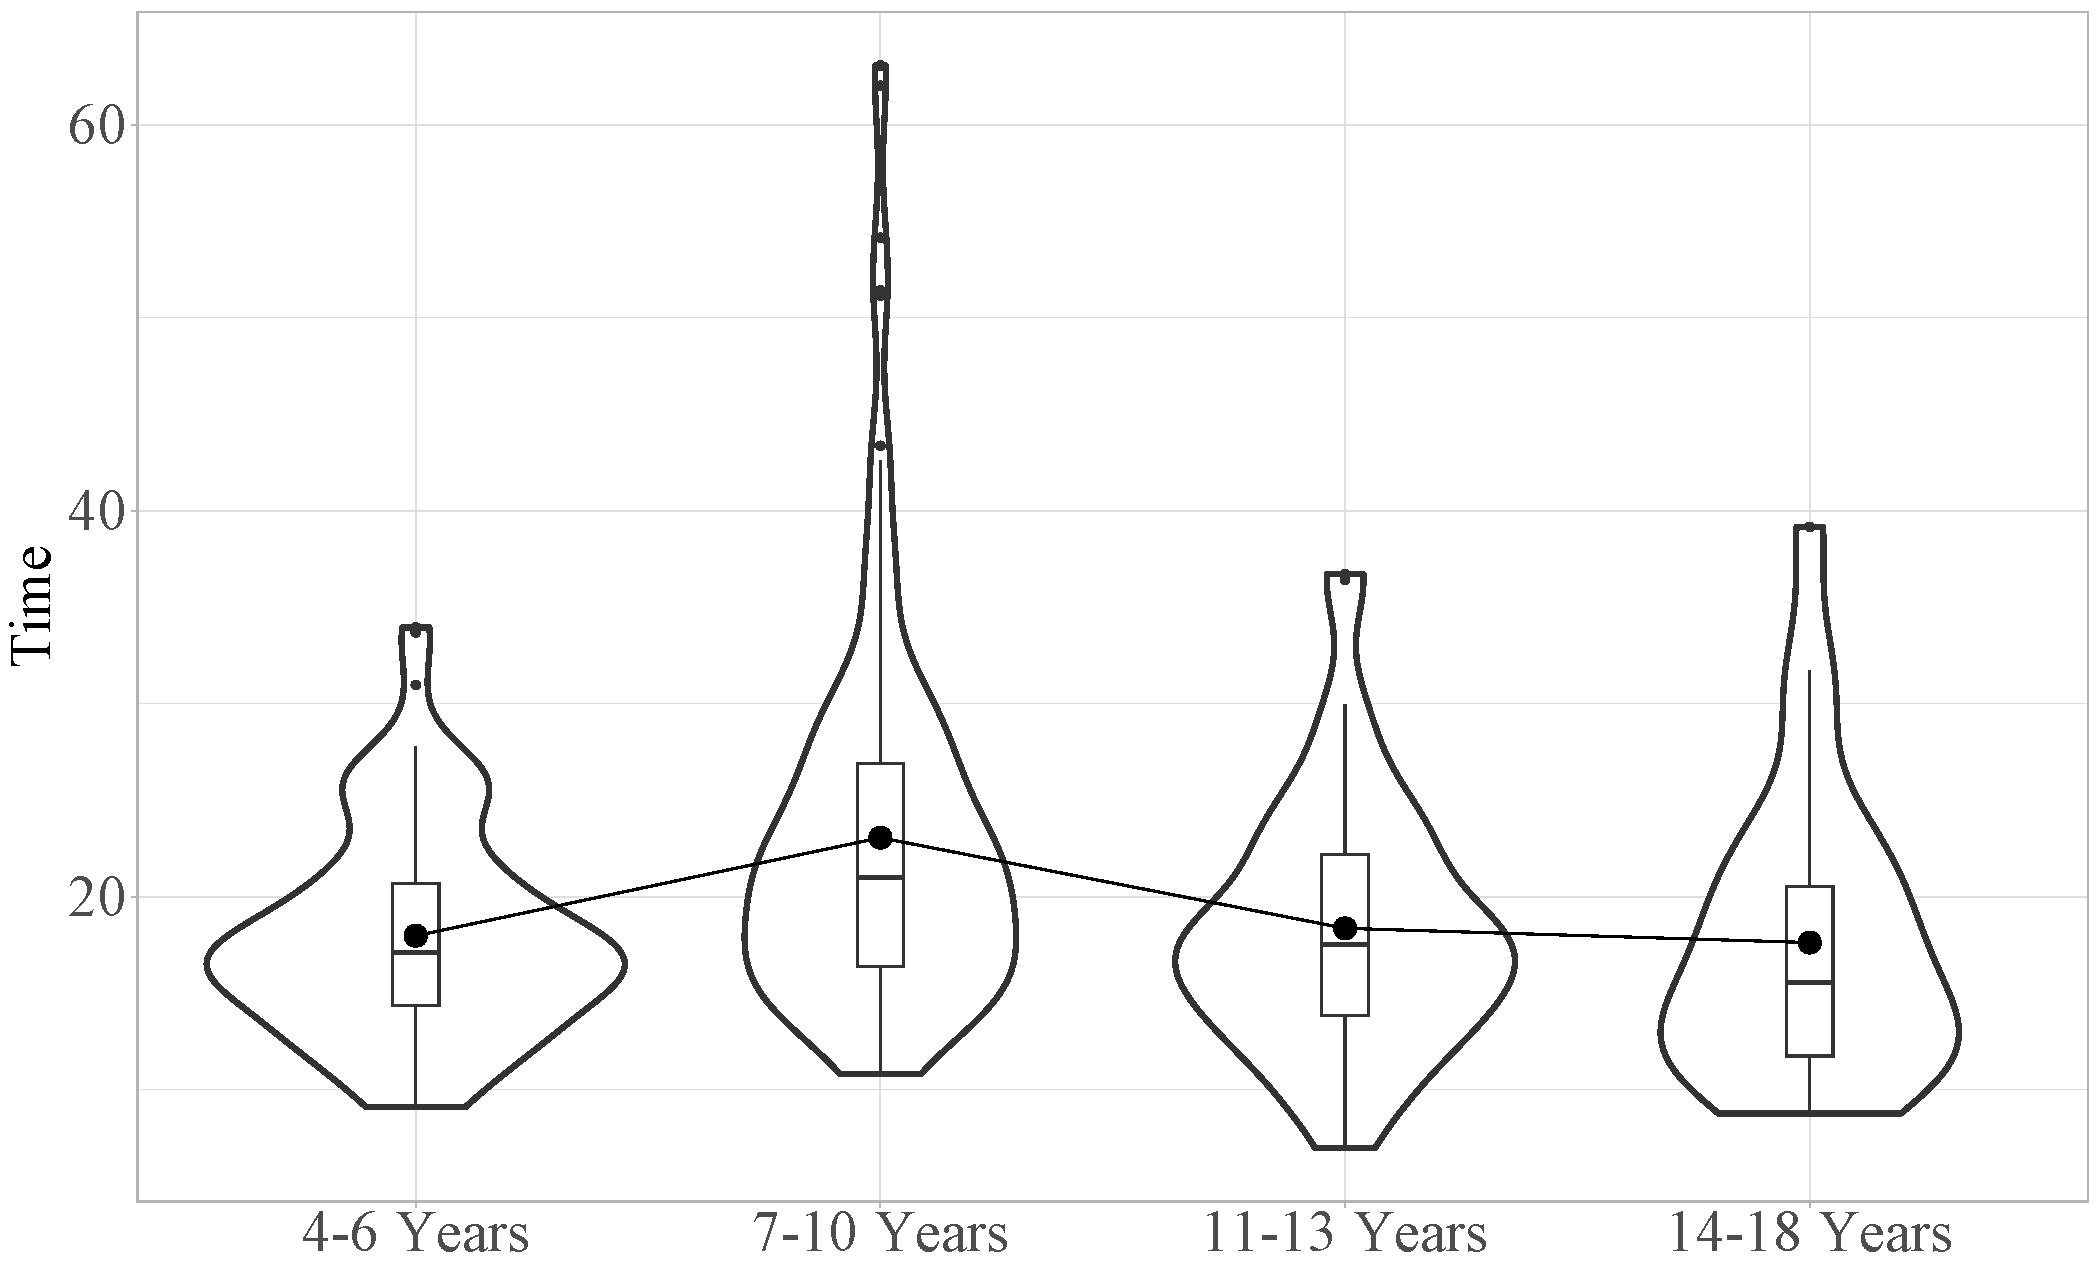
\includegraphics[width=\linewidth]{img/descrittive_tempi.pdf}
%	\end{column}
%	\end{columns}
%			\end{frame}


\begin{frame}
	
	\begin{figure}
		\centering
		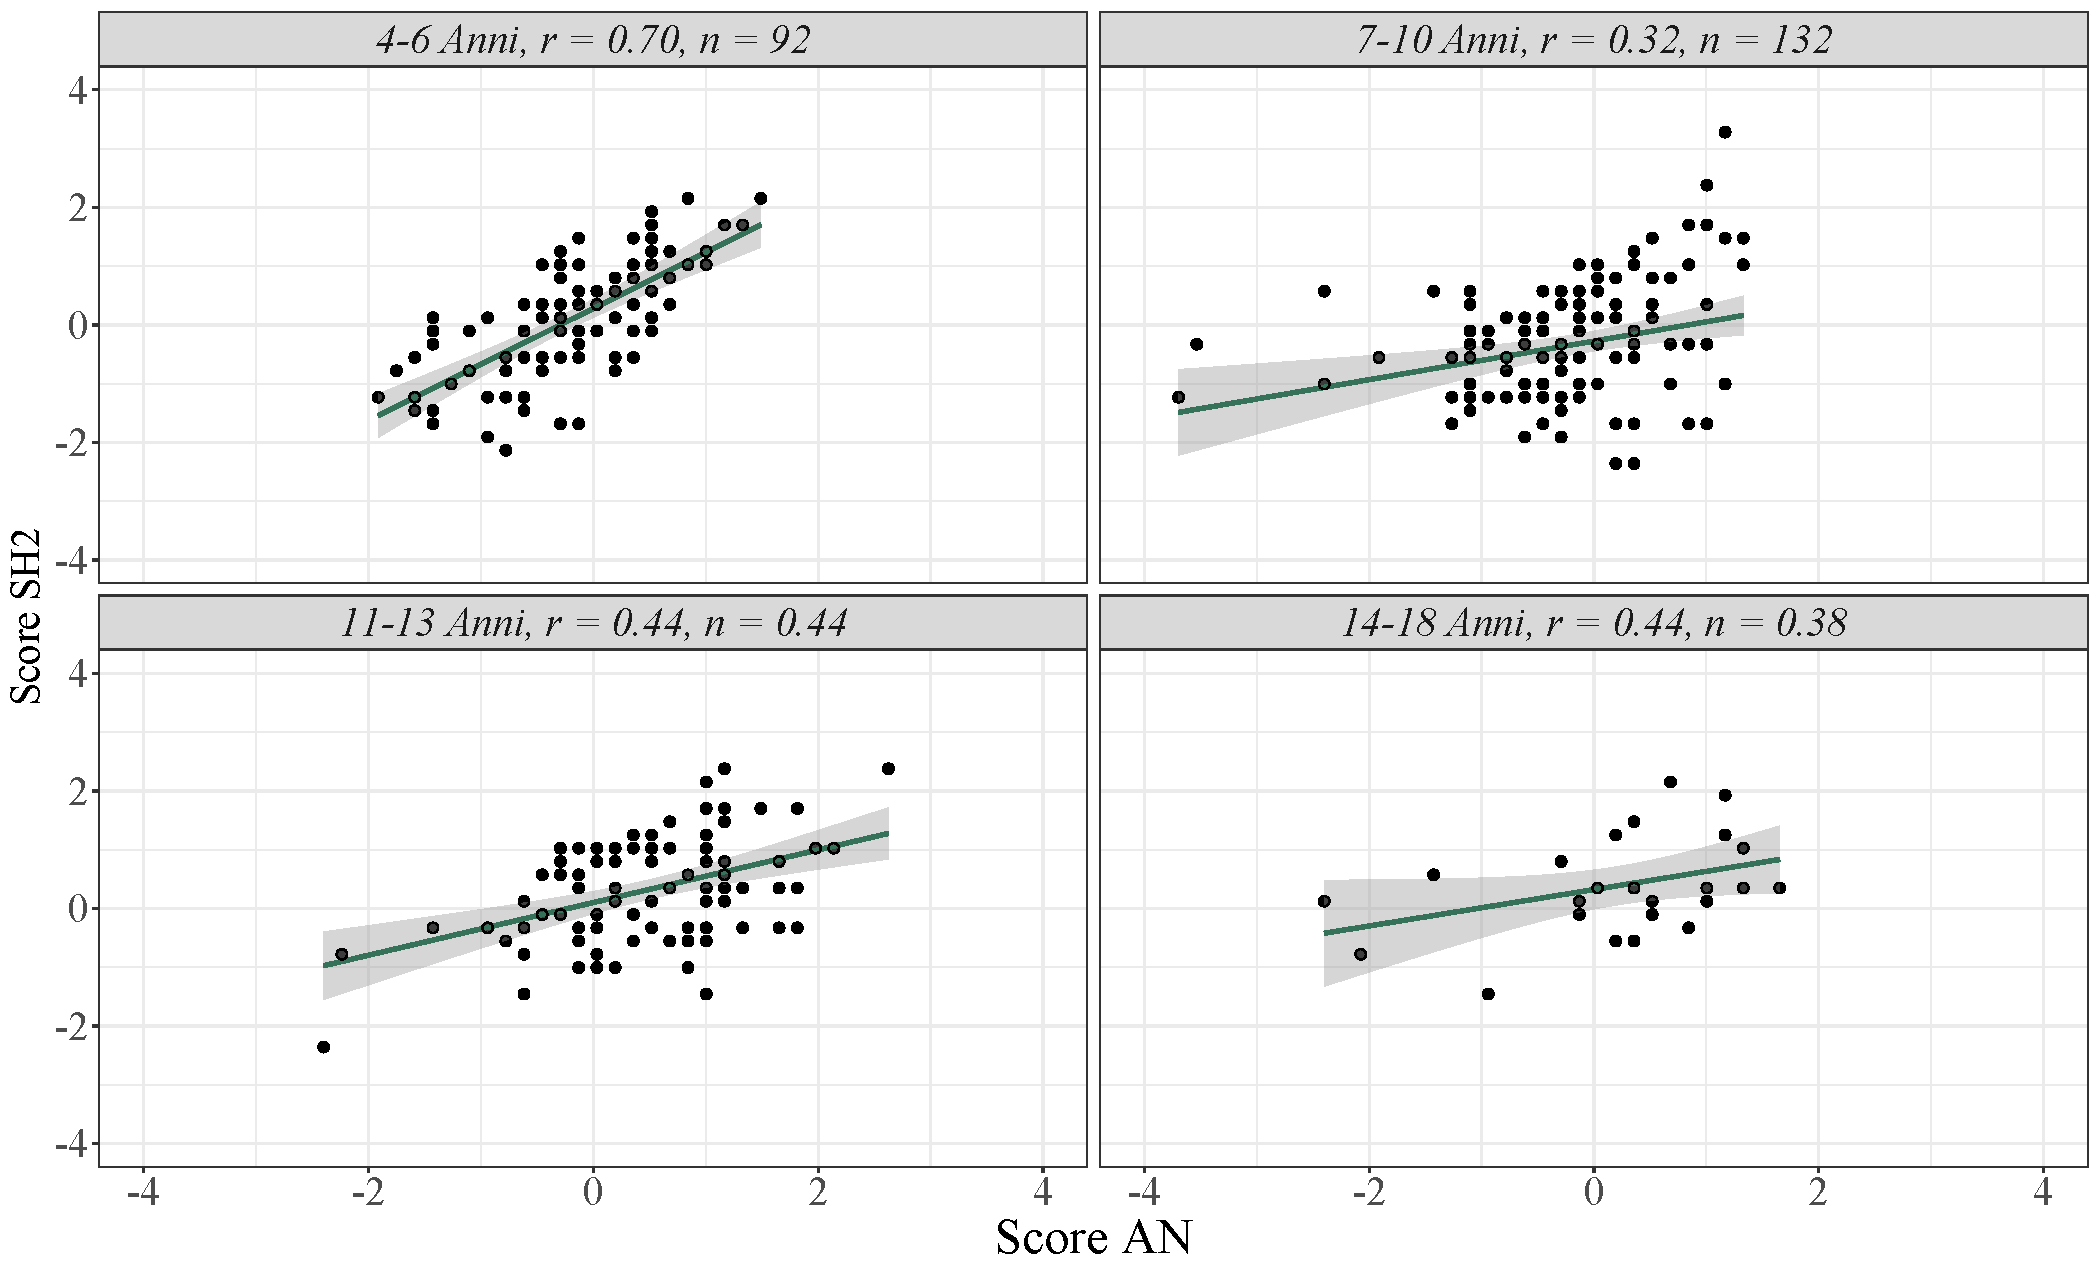
\includegraphics[width=\linewidth]{img/correlazioni_gruppi.pdf}
	\end{figure}
	
\end{frame}


\begin{frame}{Is it really bad...?}
	
Respondents  $i,j \in \{1, \ldots N\}$ 

 

\vspace{3mm}

\begin{itemize}
	
	\item  AN Comparison ($\Delta_{\text{AN}}$): The standardized AN score of each subject $i$ is compared against the standardized AN score of every other subject $j$

\begin{equation*}
 \Delta_{\text{AN}_{ij}} = z_{\text{AN}_i} - z_{\text{AN}_j}
\end{equation*}

	\item  SH2 Comparison ($\Delta_{\text{SH2}}$): The standardized SH2 score of each subject $i$ is compared against the standardized SH2 score of every other subject $j$

\begin{equation*}
\Delta_{\text{SH2}_{ij}} = z_{\text{SH2}_i} - z_{\text{SH2}_j}
\end{equation*}

\end{itemize}





\end{frame}


\begin{frame}
	\begin{overprint}
		
		\onslide<1>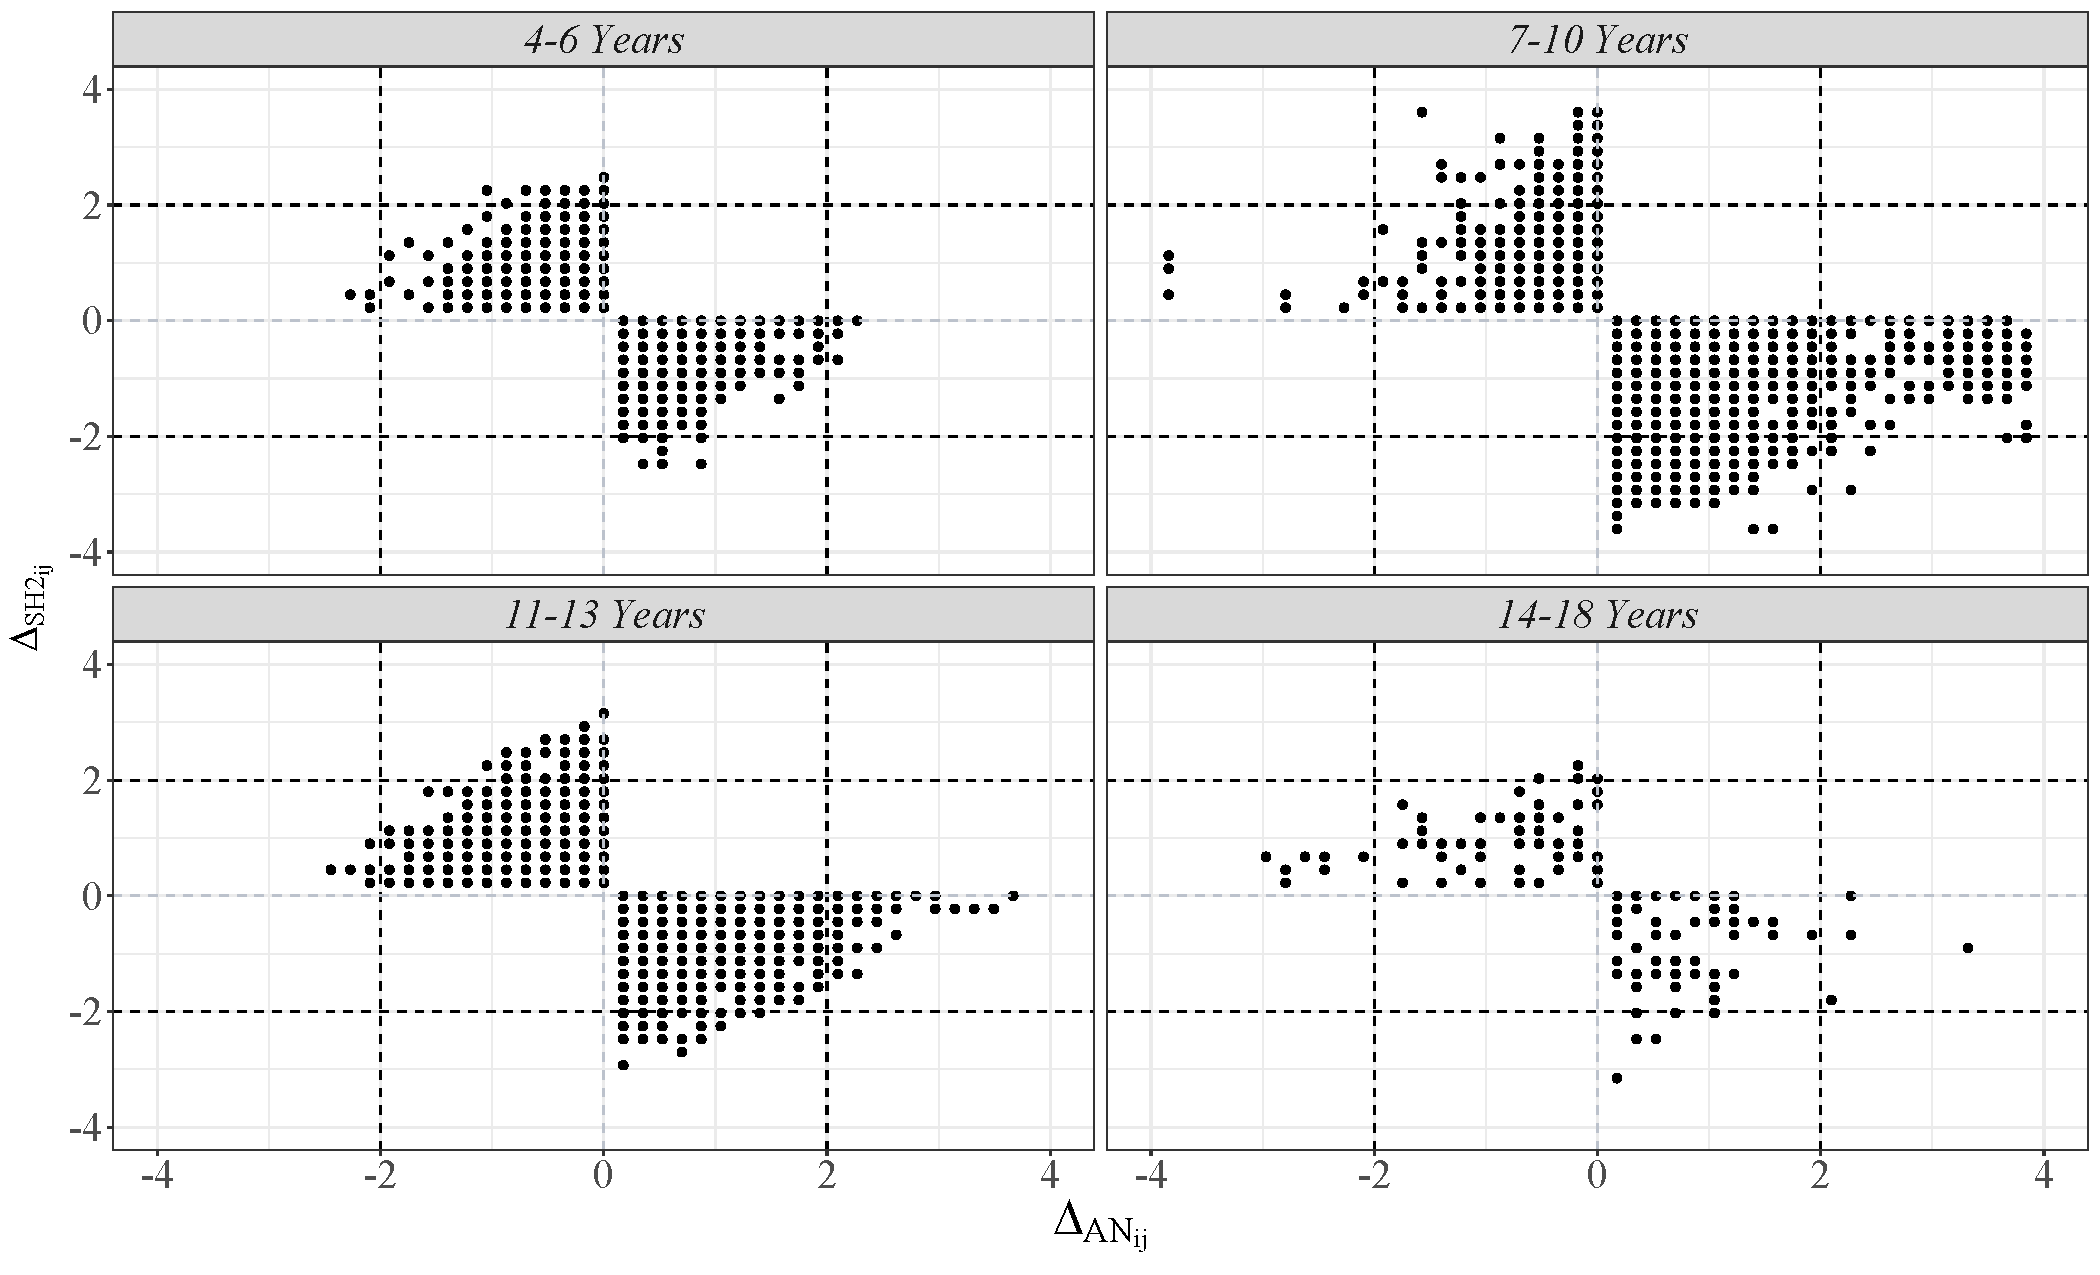
\includegraphics[width=\linewidth]{img/farfalle_gruppi.pdf}
		\onslide<2>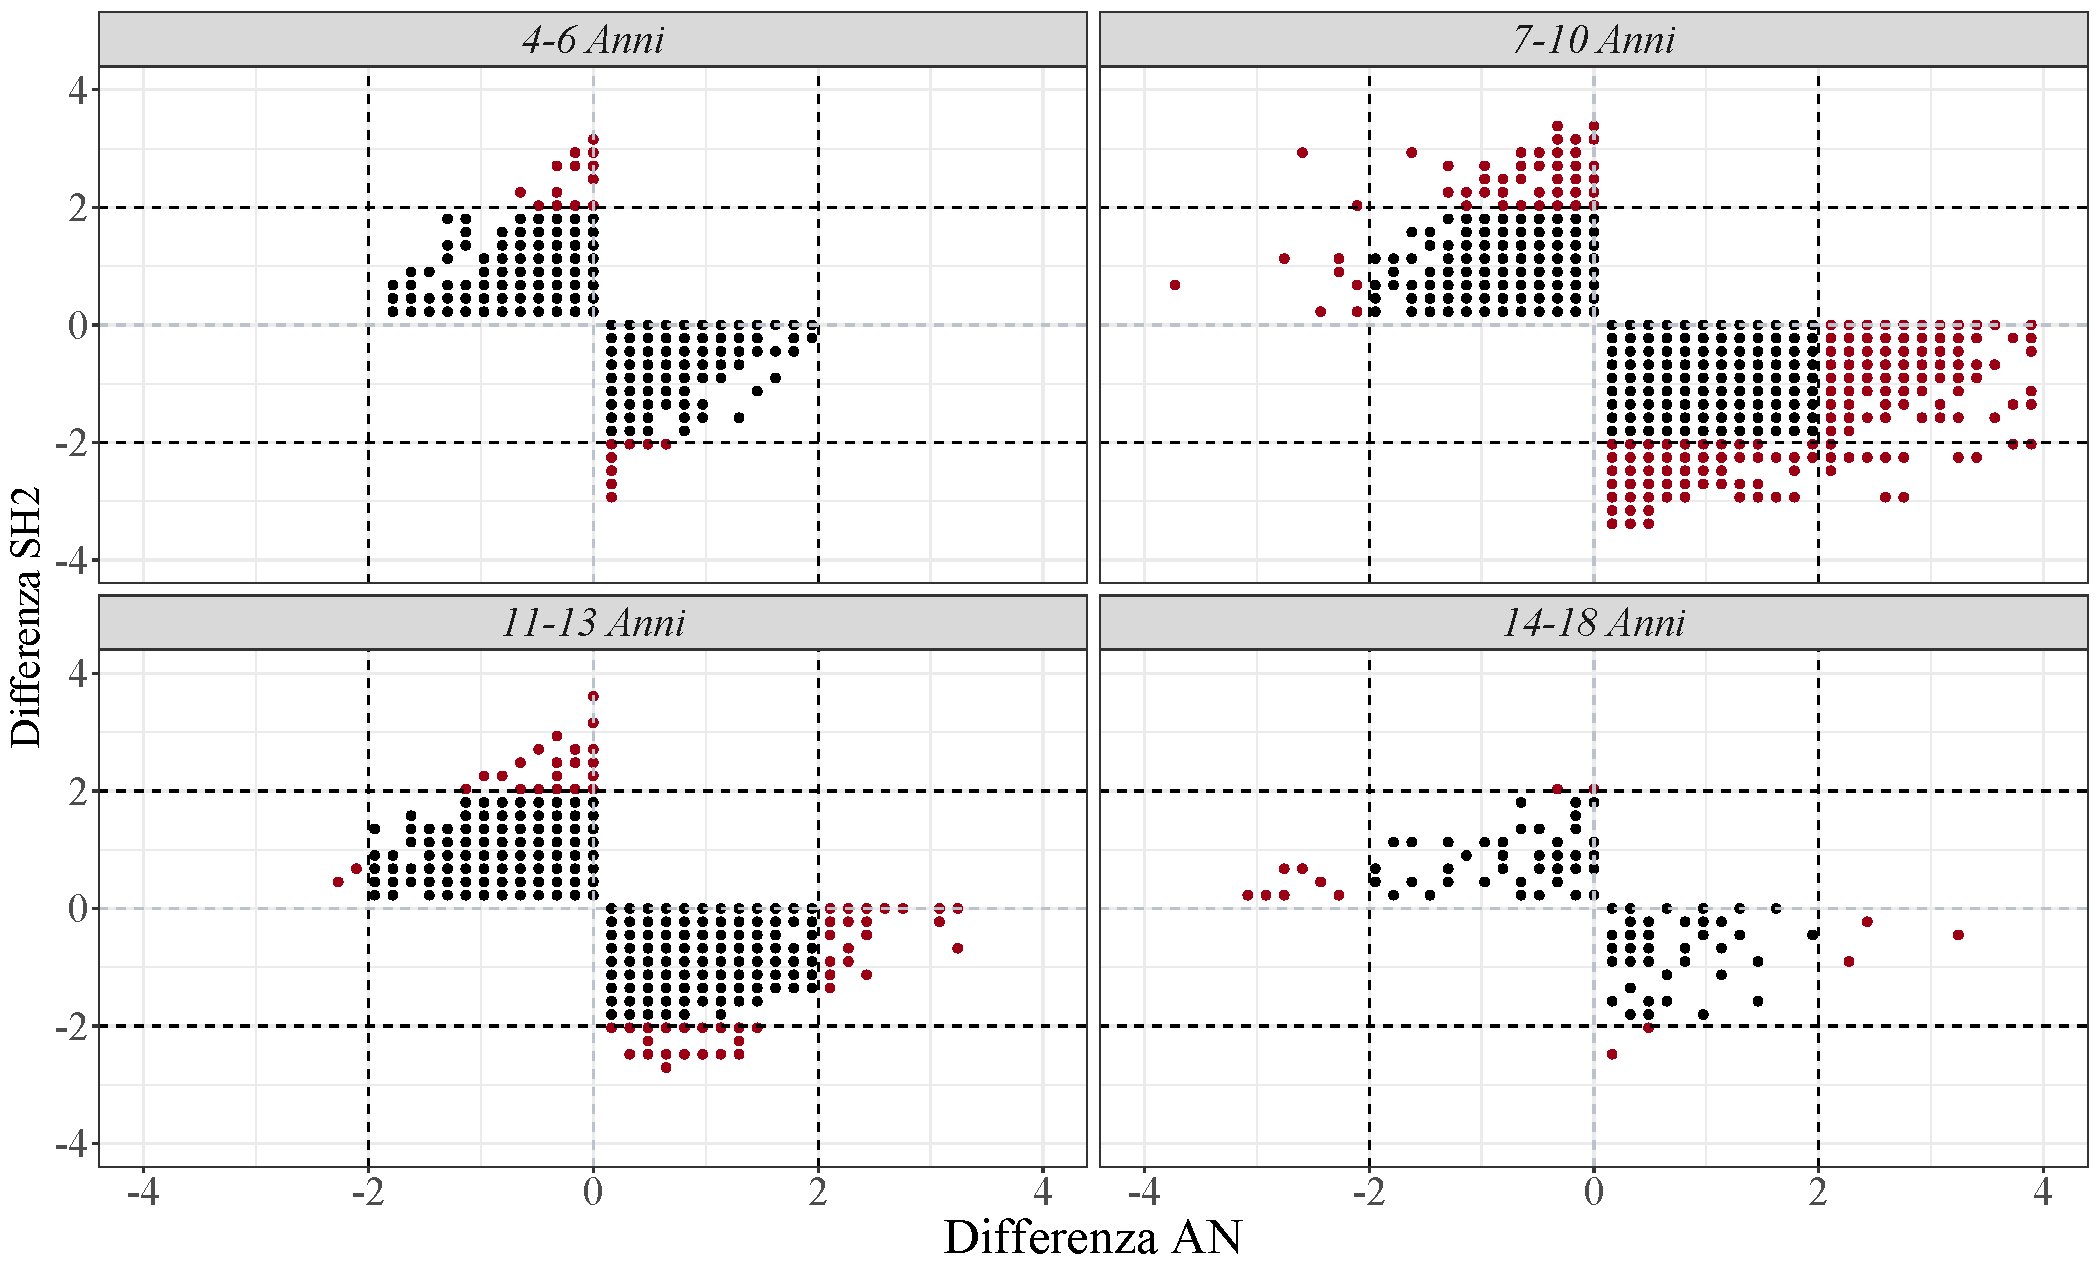
\includegraphics[width=\linewidth]{img/farfalle_gruppi_colored.pdf}

		
		
	\end{overprint}
\end{frame}


\begin{frame}
		\vspace*{-3mm}
	\begin{columns}[T]
		\begin{column}{.50\linewidth}
		
			\begin{center}
				$\Delta_{\text{AN}} > 2$ \& $\Delta_{\text{SH2}} 	\approx 0$ 
			\end{center}
		\begin{figure}
			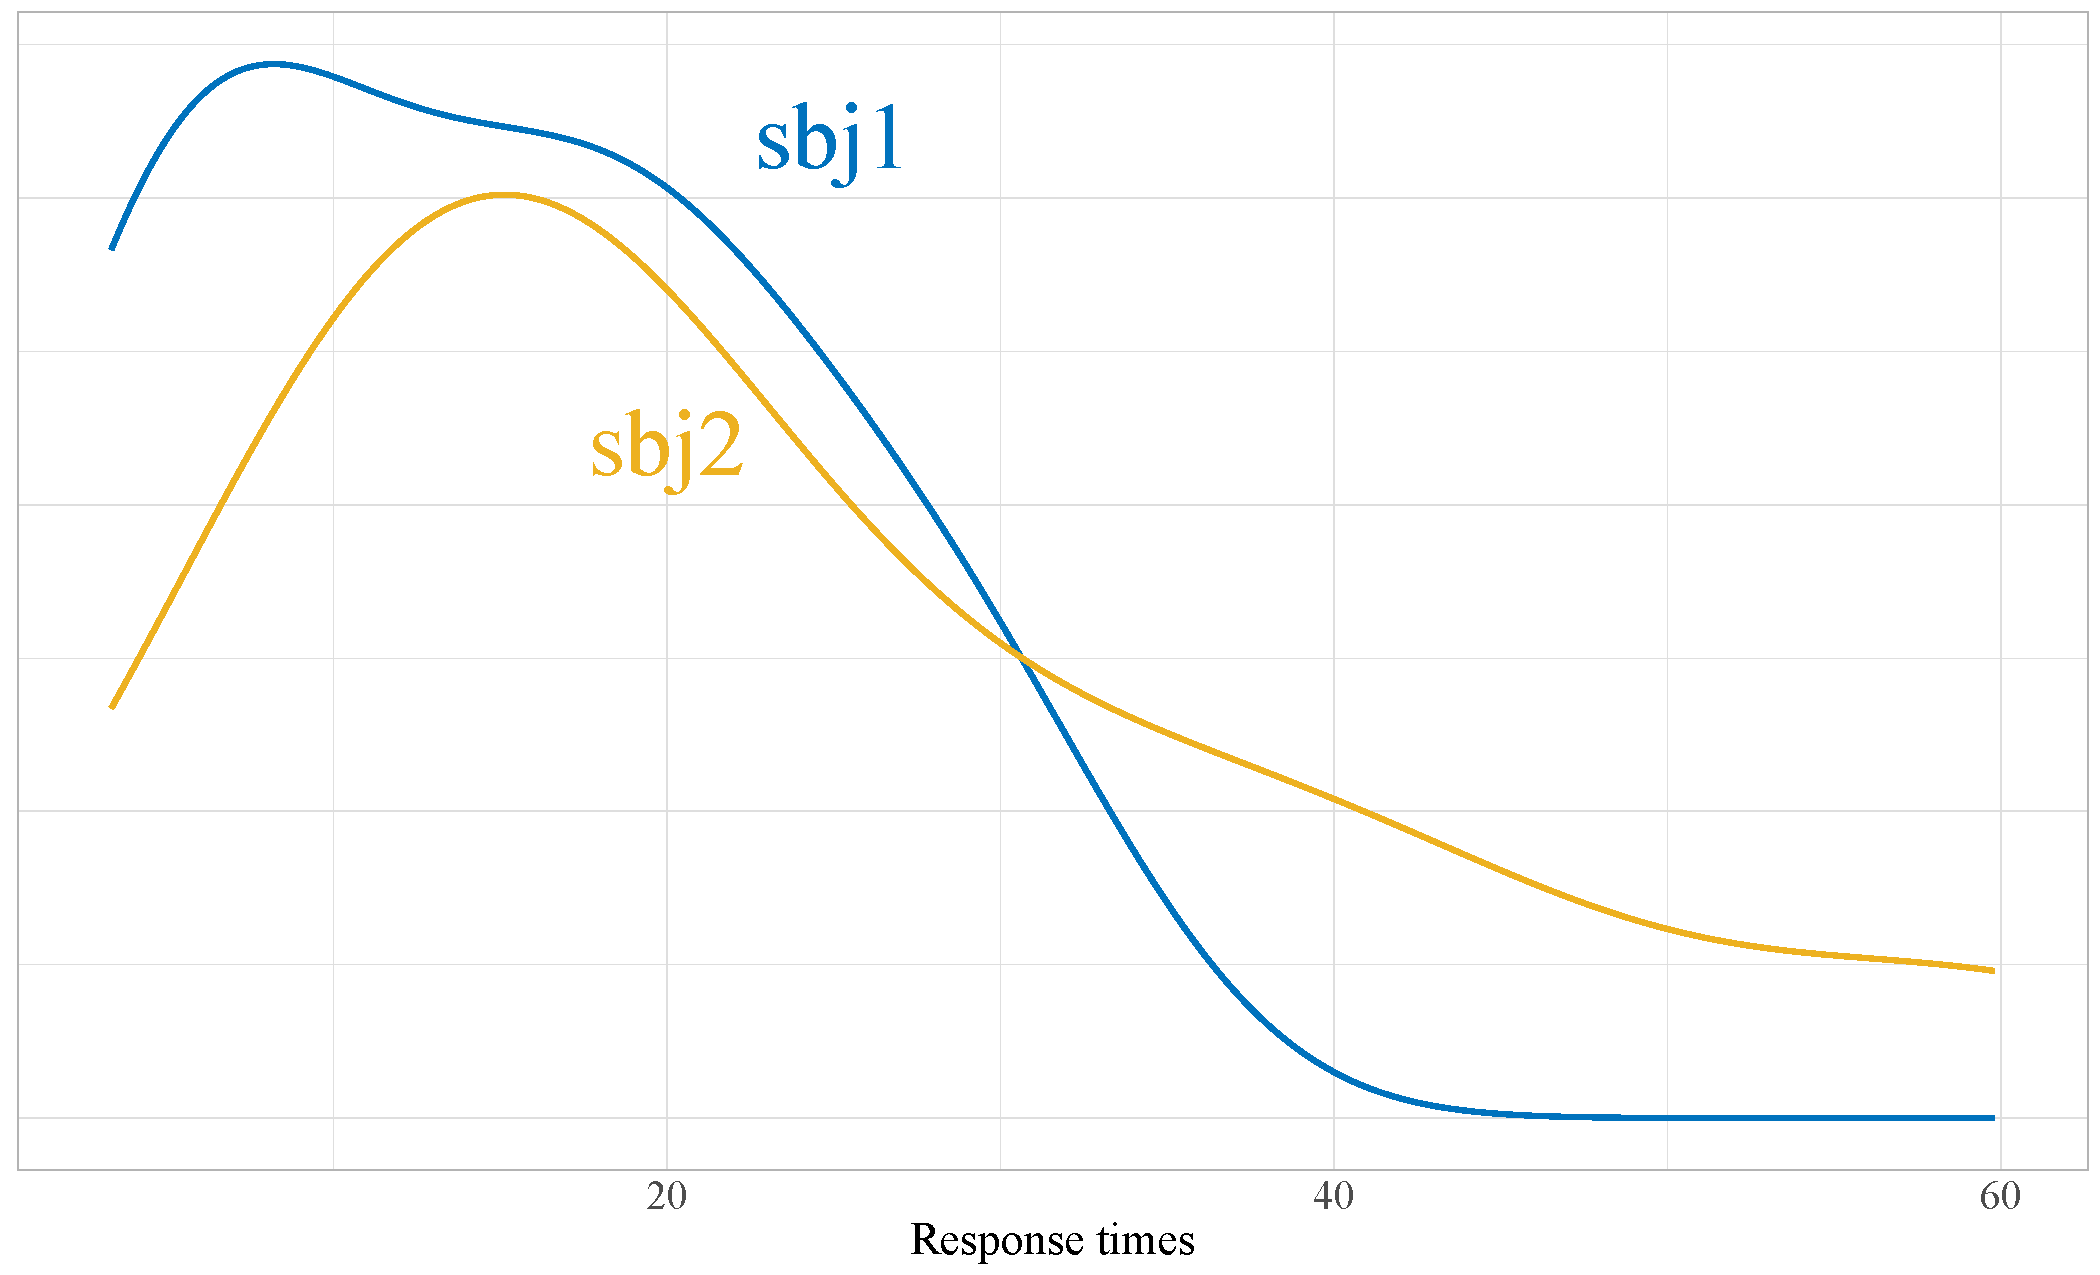
\includegraphics[width=\linewidth]{img/time_an_group_4_8.pdf}
		\end{figure}
		
		\scalebox{.55}{
					\begin{tabular}{c c c c c}
						\hline
			& $z_{\text{AN}}$ & $z_{\text{SH2}}$ & Accuracy & Time (sd) \\ \hline
						\textbf{\textcolor{sbj3}{sbj1}} & $-1.55$ & $0.43$ & 0.75&$24.10$ ($15.60$) \\	
			\textbf{\textcolor{sbj2}{sbj2}}	 & $0.72$ & $0.43$ & 0.75 &  $14.51$ ($9.22$) \\
			
			\hline
			& & & & \\\hline
			& \multicolumn{2}{c}{$\Delta_{\text{AN}}$ } & \multicolumn{2}{c}{$\Delta_{\text{SH2}}$ } \\ \hline
			\textbf{\textcolor{sbj3}{sbj1}} $-$ \textbf{\textcolor{sbj2}{sbj2}}& \multicolumn{2}{c}{$2.27$} & \multicolumn{2}{c}{$0.00$}\\\hline

		\end{tabular}
		}
			\centering

		\end{column}
			\begin{column}{.50\linewidth}
			\begin{center}
			$\Delta_{\text{AN}} \approx 0$ \& $\Delta_{\text{SH2}}  > 2 $ 
		\end{center}
		\begin{figure}
			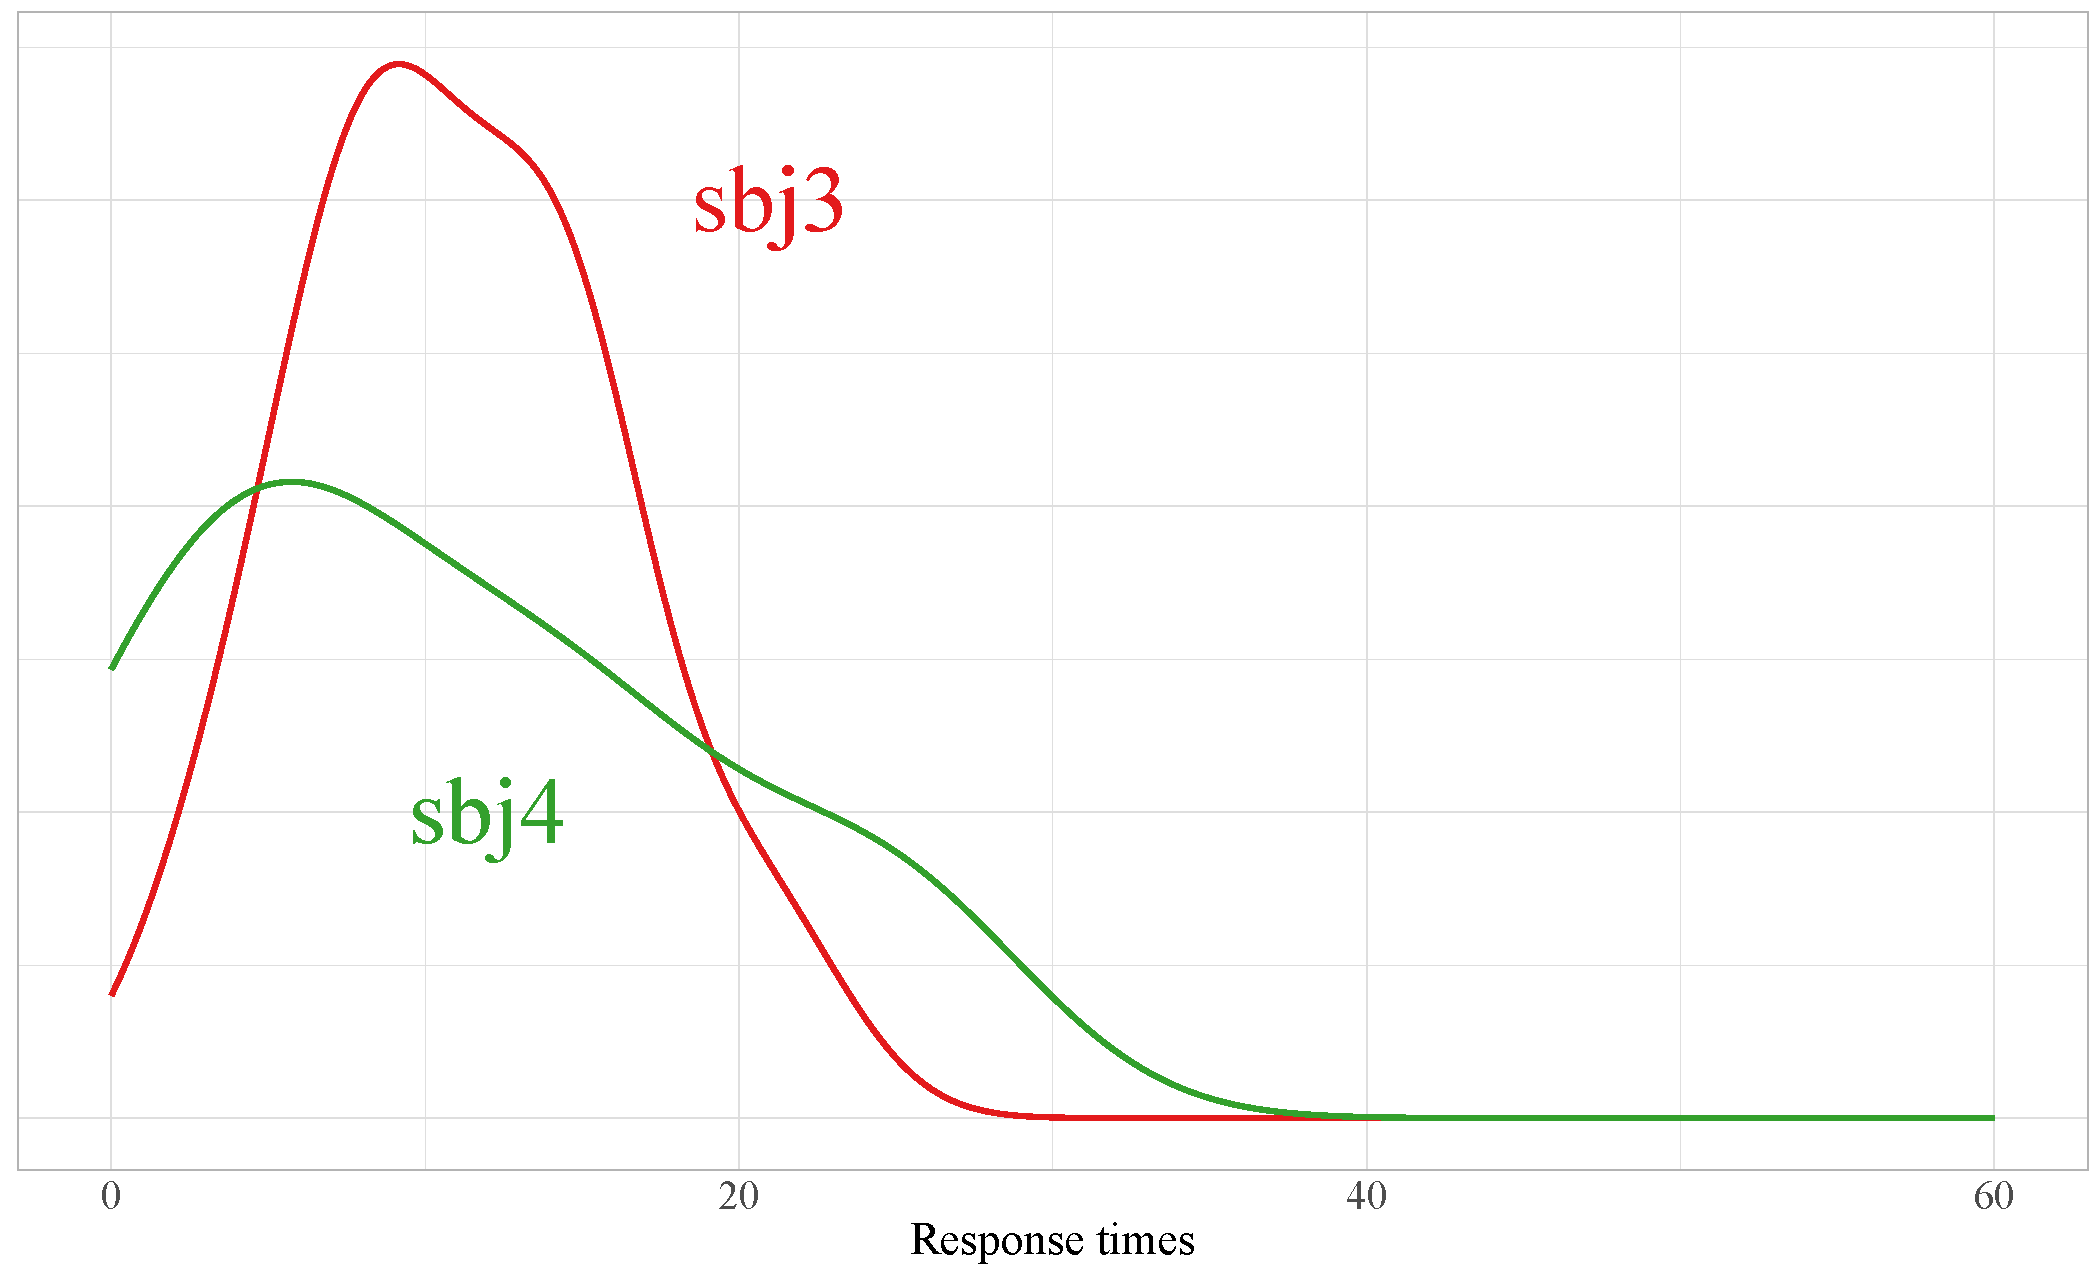
\includegraphics[width=\linewidth]{img/time_sh_group_4_8.pdf}
		\end{figure}
		\scalebox{.55}{
			\begin{tabular}{c c c c c}
				\hline
				& $z_{\text{AN}}$ & $z_{\text{SH2}}$ & Accuracy & Time (sd) \\ \hline
				\textbf{\textcolor{sbj6}{sbj3}}	 & $-0.15$ & $1.55$ & 0.75 & $11.14$ ($4.96$) \\
				\textbf{\textcolor{sbj5}{sbj4}} & $0.20$ & $-0.70$ & 0.58& $10.72$ ($8.60$)\\				
				\hline
				& & & & \\\hline
				& \multicolumn{2}{c}{$\Delta_{\text{AN}}$ } & \multicolumn{2}{c}{$\Delta_{\text{SH2}}$ } \\ \hline
				\textbf{\textcolor{sbj6}{sbj3}} $-$ \textbf{\textcolor{sbj5}{sbj4}}& \multicolumn{2}{c}{$-0.35$} & \multicolumn{2}{c}{$2.25$}\\\hline
				
			\end{tabular}
		}
		\end{column}
	\end{columns}
\end{frame}

\section{Final remarks}

\begin{frame}
	
	\begin{block}{Highlights}
		
		\begin{itemize}
			\item Different scoring systems $\rightarrow$ The focus is shifted: Fast and furious or slow and steady?
			\item Different scoring systems might favor a cognitive theory over a contrasting one (raising also replicability issues)
		\end{itemize}
	\end{block}
	
	
	\vspace{20mm}
	\scriptsize
	Research founded by the project ``Computerized, Adaptive and Personalized Assessment of Executive Functions and Fluid Intelligence''
(PRIN 2020, Prot. 20209WKCLL, P.I. Prof. Luca Stefanutti)
	
\end{frame}

\begin{frame}[plain]

\begin{figure}
\centering

\includegraphics[width=.30\linewidth]{img/qr-code.png}
\end{figure}



	\centering
	
	\Large
	Thank you!
	\normalsize
	
	\vspace{3mm}
	ottavia.epifania@unipd.it
\end{frame}
 
\end{document}